\section*{Empirical Results}

\subsection*{Modeling Procedure and Implementation}
The empirical implementation relies on a custom-built \texttt{Python} function designed to estimate log-linear hedonic regression models with enhanced robustness and flexibility. The function integrates tools from \texttt{statsmodels} and \texttt{scikit-learn} to streamline the modeling pipeline. In addition to the linear specification, a separate function was developed to estimate GAM, allowing for nonlinear relationships between selected predictors and the logarithm of sale price. The GAM function utilizes the \texttt{pyGAM} library and incorporates cross-validation for hyperparameter tuning, enabling flexible smoothing of continuous variables while retaining linear treatment of categorical features. Below the results of both the linear and additive hedonic pricing models for residential properties are presented, describing how each was built and refined.


\subsubsection*{Geographic Units of Analysis: Central and East Orlando}
To examine potential spatial heterogeneity in housing attribute valuation, the hedonic model was estimated separately for two Orlando areas. Central Orlando includes ZIP codes $32801$, $32804$, $32806$, $32807$, $32809$, $32812$, $32822$, and $32839$. These ZIP codes correspond to neighborhoods largely within the administrative boundaries of the City of Orlando, including prominent areas such as Downtown Orlando, College Park, Edgewood, Lake Eola Heights, Park Central, and Azalea Park. The area is characterized by a heterogeneous housing stock, including a significant share of older homes constructed in the mid-20th century. This region exhibits median home prices ranging approximately from $\$260,000$ to $\$570,000$, reflecting a broad spectrum of property types, from standard newly constructed houses to historic residences in established neighborhoods such as Lake Como, Colonialtown, and Downtown Orlando. The average population density in this region is approximately 4890 people per square mile, indicating relatively high levels of urbanization.

East Orlando includes ZIP codes $32817$, $32820$, $32826$, and $32828$. This area lies outside the official city limits and represent a more suburban landscape, with extensive residential development occurring primarily from the 1980s onward. It is characterized by large, planned communities such as Avalon Park and Waterford Lakes, along with neighborhoods like Union Park, Alafaya, and the area surrounding the University of Central Florida. The housing stock is more homogeneous, with many properties located within planned subdivisions and exhibiting modern construction standards and layouts. Median home prices in this area range between $\$370,000$ and $\$480,000$, suggesting a relatively narrower distribution compared to Central Orlando. With an average population density of 2440 people per square mile, the region features lower development intensity and greater separation between residential and commercial zones.

Estimating the hedonic model separately across these two regions facilitates comparison of buyer's valuations of structural and neighborhood attributes under distinct urban development contexts.

\subsubsection*{Regularization-Based Feature Selection with LASSO}

To enhance the model's applicability across diverse geographical regions, feature selection is dynamically performed using LASSO regularization. Due to heterogeneity across different housing markets, it is expected that varying attributes will predominantly drive housing prices in different locations. LASSO regression addresses this by penalizing coefficients towards zero, selectively retaining only the most impactful features that significantly contribute to housing prices. 


Following feature selection, the retained subset of variables can be expressed as:
\[
\widehat{S} = \left\{ j \in \{1, \dots, J\} \; : \; \hat{\beta}^{\text{LASSO}}_j \neq 0 \right\}
\]
\noindent where $\widehat{S}$ is the set of indices for predictors retained by the LASSO model. 

\begin{table}
\caption{LASSO Feature Selection Results by Region}
\label{tab:lasso_selection_results}
\begin{tabular}{lll}
\toprule
Feature & Selected: Orlando Central & Selected: Orlando East \\
\midrule
Home Type & Home Type & Home Type \\
Age of Property & Age of Property & Age of Property \\
Bedrooms & Bedrooms & Bedrooms \\
Bathrooms & Bathrooms & Bathrooms \\
Sq. Feet per Bedroom & Sq. Feet per Bedroom & Sq. Feet per Bedroom \\
Number of Stories &  & Number of Stories \\
Number of Parking Spaces &  &  \\
Garage & Garage & Garage \\
Private Pool & Private Pool & Private Pool \\
HOA & HOA & HOA \\
Gated Community & Gated Community & Gated Community \\
Recreational Facilities &  &  \\
Nearby Park & Nearby Park &  \\
Playground Nearby & Playground Nearby & Playground Nearby \\
Greenbelt &  &  \\
Above Flood Plain & Above Flood Plain & Above Flood Plain \\
City Lot & City Lot &  \\
Historic District &  &  \\
Water View & Water View & Water View \\
Average Distance to Schools &  &  \\
Average School Rating & Average School Rating & Average School Rating \\
Min. Distance to Highway & Min. Distance to Highway & Min. Distance to Highway \\
\bottomrule
\end{tabular}
\end{table}



Although LASSO is effective for variable selection, it introduces bias by shrinking coefficients and places the estimated parameter vector on the boundary of the parameter space. As a result, it violates regularity conditions required for standard asymptotic inference, making $t$-statistics, $p$-values, and confidence intervals from the LASSO estimates unreliable \citep{lockhartEtAl:2014}. To enable valid statistical inference, the final step involves re-estimating the least squares model using only the subset of predictors selected by LASSO. This methodology helps in dynamically adapting the model to regional variations while maintaining a robust and interpretable structure.



\subsection*{Model Performance of Least Squares}

\subsubsection*{Model Fit}
The log-linear regression models for Central Orlando and East Orlando demonstrate strong overall fit and predictive accuracy, with $R^2$ values of $0.839$ and $0.920$, respectively. The Root Mean Squared Error (RMSE) is $0.194$ for Central Orlando and $0.087$ for East Orlando, reflecting the average squared prediction error in logarithm of sale prices. These results suggest that a substantial portion of the variation in logarithm of sale prices is explained by the selected housing and neighborhood attributes. Given that the models did not incorporates granular interior features or detailed exterior characteristics, these results reflect a high degree of explanatory power. The overall F-statistics confirm that the models are jointly significant.


\begin{table}[H]
\centering
\caption{Least-Squares Model Fit Statistics: Central Orlando and East Orlando}
\label{tab:model_comparison}
\begin{tabular}{lcc}
\toprule
& \textbf{Orlando Central} & \textbf{Orlando East} \\
\midrule
R-squared           & 0.839  & 0.920 \\
F-statistic                    & 675.9  & 649.3 \\
p-value (F-statistic)          & 0.000  & 0.000 \\
RMSE  & 0.194 & 0.087 \\
\bottomrule
\end{tabular}
\end{table}

\subsubsection*{Residual Diagnostics}

The normality assumption in linear regression requires that the error terms are normally distributed with mean zero and constant variance:

\[
U_n \sim \mathcal{N}(0, \sigma^2)
\]

\noindent This assumption underpins the validity of statistical inference in the method of least squares regression, including confidence intervals and hypothesis tests.


\begin{figure}[H]
	\centering
	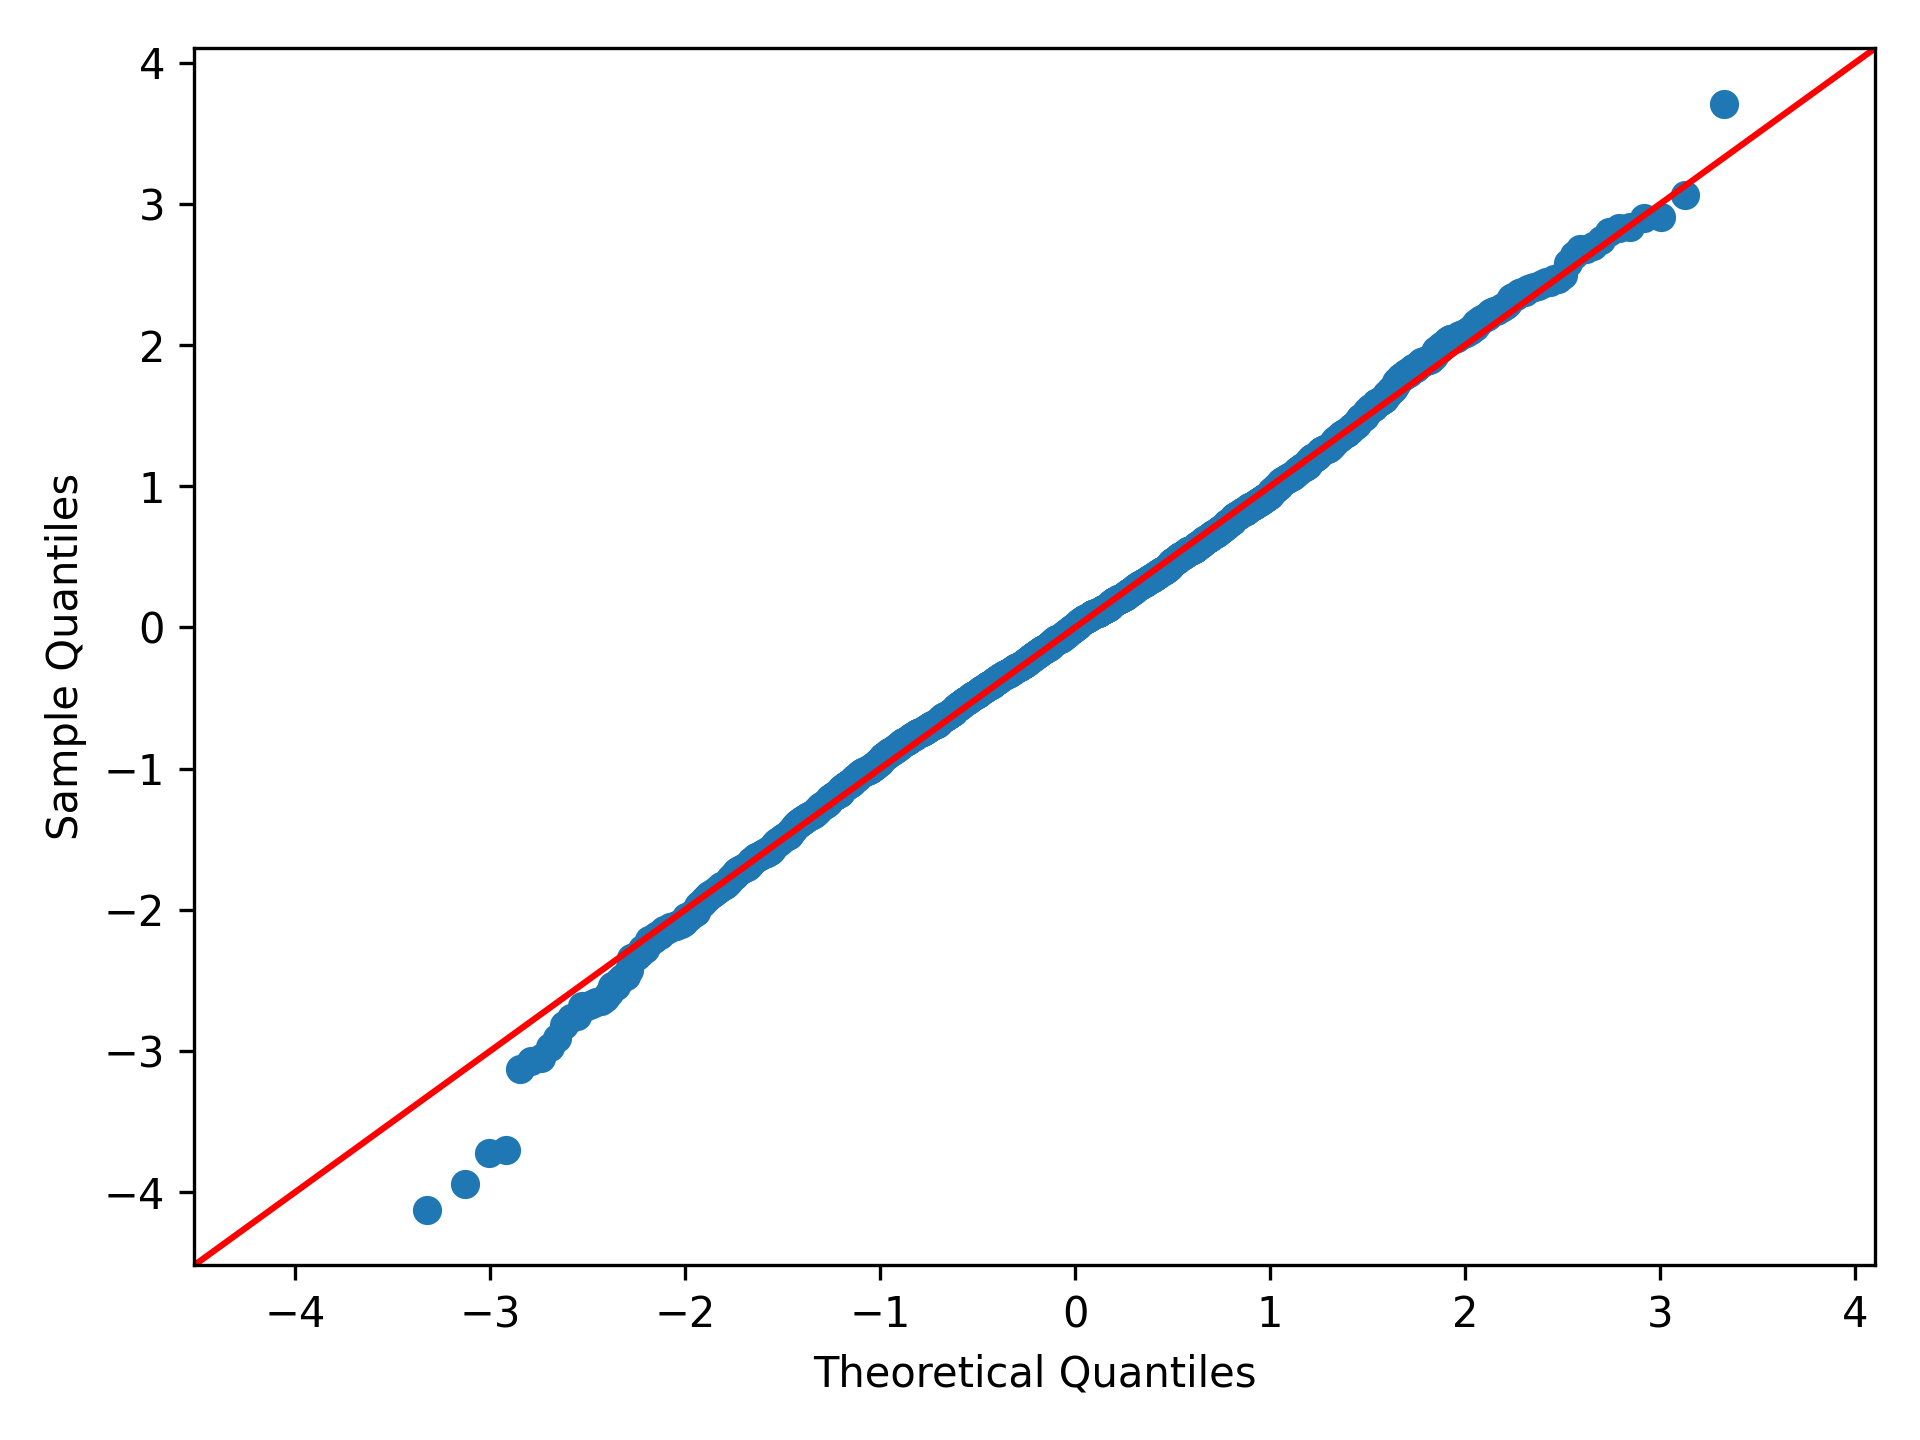
\includegraphics[width=0.7\textwidth]{Figures/qqplot_orlando_central.png}
    \caption{Plot of Residuals for Central Orlando}
	\label{fig:2}
\end{figure}

\begin{figure}[H]
	\centering
	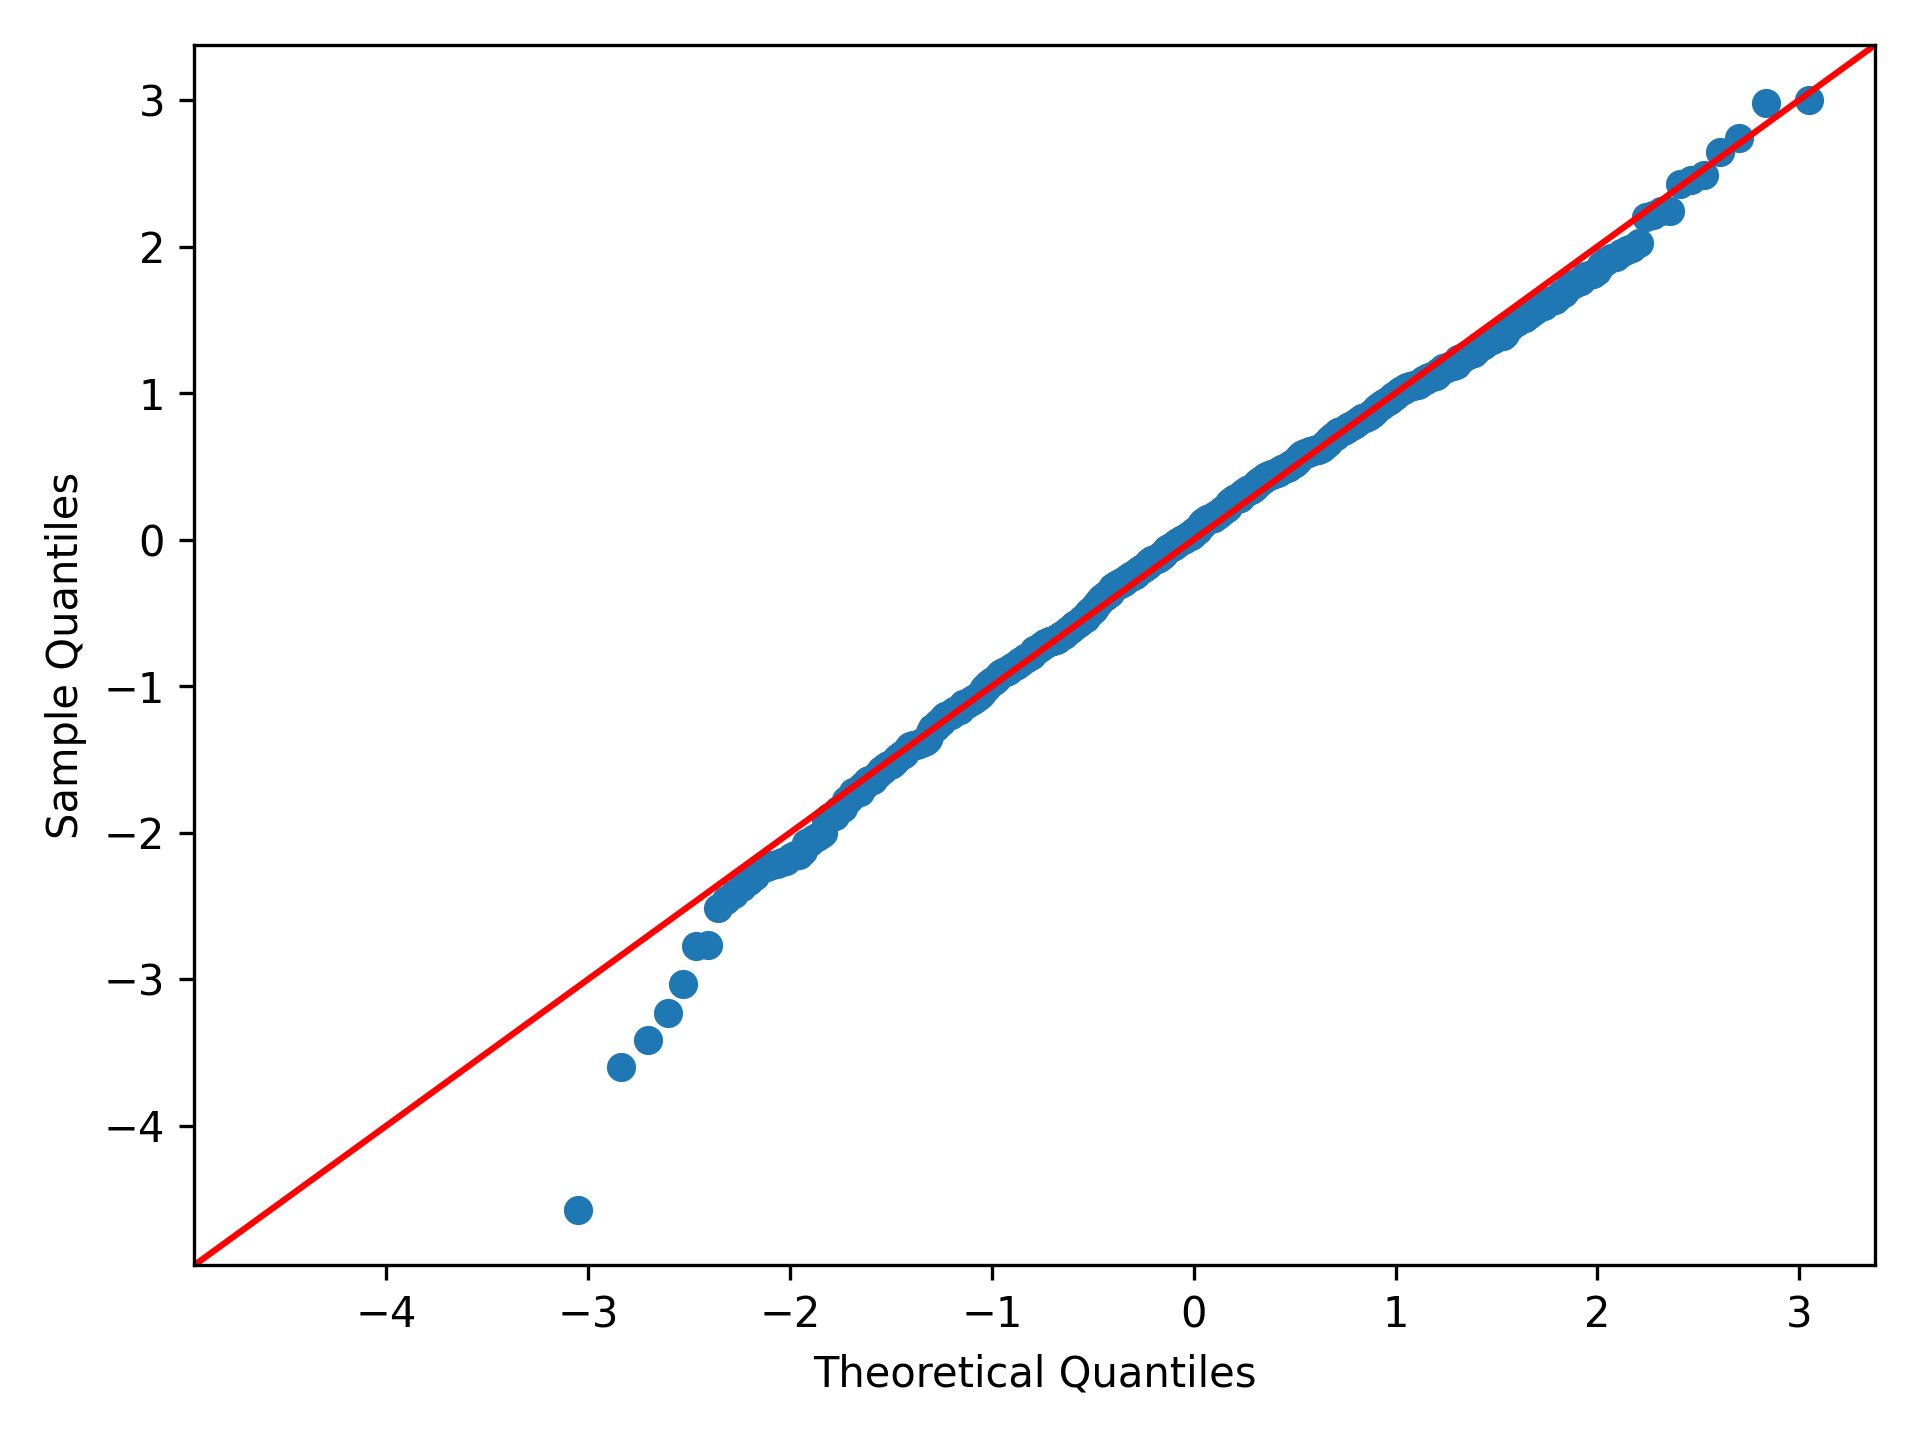
\includegraphics[width=0.7\textwidth]{Figures/qqplot_orlando_east.png}
    \caption{Plot of Residuals for East Orlando}
	\label{fig:3}
\end{figure}


To evaluate whether the residuals satisfy the normality assumption, a Q–Q (quantile–quantile) plot is used to visually compare the empirical distribution of residuals to a theoretical normal distribution. As shown in Figure~\ref{fig:2} and Figure~\ref{fig:3}, the residuals generally align with the 45-degree reference line, with only some deviations in the tails. This suggests that the residuals are approximately normally distributed, supporting the validity of least squares regression inference procedures.

\subsubsection*{Parameter Estimates}


\begin{table}
\caption{Least‑Squares Estimates with 95 percent CI (Central Orlando)}
\label{tab:ols_coeffs_c}
\begin{tabular}{lrrrr}
\toprule
 & Coefficient & Std. Error & CI Lower & CI Upper \\
\midrule
const & 7.4615 & 0.1436 & 7.1800 & 7.7430 \\
Sq. Feet per Bedroom & 0.6664 & 0.0231 & 0.6211 & 0.7117 \\
Home Type & 0.1856 & 0.0085 & 0.1690 & 0.2023 \\
Bedrooms & 0.1851 & 0.0085 & 0.1685 & 0.2017 \\
City Lot & 0.1249 & 0.0136 & 0.0983 & 0.1516 \\
Garage & 0.1089 & 0.0109 & 0.0875 & 0.1302 \\
Above Flood Plain & 0.0850 & 0.0223 & 0.0413 & 0.1287 \\
Bathrooms & 0.0837 & 0.0096 & 0.0649 & 0.1026 \\
Private Pool & 0.0724 & 0.0116 & 0.0496 & 0.0952 \\
Nearby Park & 0.0629 & 0.0150 & 0.0335 & 0.0922 \\
Water View & 0.0512 & 0.0148 & 0.0222 & 0.0802 \\
Average School Rating & 0.0312 & 0.0055 & 0.0205 & 0.0419 \\
Playground Nearby & 0.0254 & 0.0117 & 0.0025 & 0.0483 \\
Gated Community & -0.0165 & 0.0122 & -0.0403 & 0.0074 \\
Age of Property & -0.0224 & 0.0030 & -0.0283 & -0.0166 \\
Min. Distance to Highway & -0.0335 & 0.0054 & -0.0440 & -0.0230 \\
HOA & -0.0997 & 0.0105 & -0.1203 & -0.0792 \\
\bottomrule
\end{tabular}
\end{table}

\begin{table}
\caption{Least‑Squares Estimates with 95 percent CI (East Orlando)}
\label{tab:ols_coeffs_e}
\begin{tabular}{lrrrr}
\toprule
 & Coefficient & Std. Error & CI Lower & CI Upper \\
\midrule
const & 9.3649 & 0.1032 & 9.1626 & 9.5672 \\
Sq. Feet per Bedroom & 0.4329 & 0.0169 & 0.3997 & 0.4661 \\
Home Type & 0.1380 & 0.0108 & 0.1168 & 0.1592 \\
Bedrooms & 0.1238 & 0.0055 & 0.1131 & 0.1345 \\
Private Pool & 0.1188 & 0.0081 & 0.1028 & 0.1347 \\
Above Flood Plain & 0.0811 & 0.0180 & 0.0458 & 0.1165 \\
Garage & 0.0744 & 0.0122 & 0.0505 & 0.0983 \\
Bathrooms & 0.0528 & 0.0076 & 0.0380 & 0.0677 \\
Gated Community & 0.0508 & 0.0110 & 0.0293 & 0.0723 \\
Water View & 0.0379 & 0.0095 & 0.0193 & 0.0565 \\
Average School Rating & 0.0237 & 0.0040 & 0.0159 & 0.0316 \\
Min. Distance to Highway & 0.0145 & 0.0021 & 0.0104 & 0.0185 \\
Playground Nearby & 0.0117 & 0.0073 & -0.0026 & 0.0261 \\
Age of Property & -0.0340 & 0.0027 & -0.0393 & -0.0286 \\
HOA & -0.0526 & 0.0075 & -0.0673 & -0.0379 \\
Number of Stories & -0.0810 & 0.0088 & -0.0982 & -0.0638 \\
\bottomrule
\end{tabular}
\end{table}


The majority of individual coefficients are statistically significant at the $5$ percent level, as shown in Table~~\ref{tab:ols_coeffs_c} and Table~~\ref{tab:ols_coeffs_e}, indicating that their estimated effects on the expected logarithm of sale price are unlikely to be the result of random variation under the null hypothesis of no association.  Reported standard errors are heteroskedasticity-consistent, improving inference in the presence of non-constant error variance. The associated confidence intervals are reasonably narrow, suggesting that the coefficient estimates are stable and estimated with precision.

\subsection*{GAM Model Performance}

\subsubsection*{Model Fit}
To capture potential nonlinearities and diminishing marginal effects common in the housing market, the analysis is extended by using GAM. Housing markets often exhibit complex, non-monotonic relationships, making GAM an appropriate tool for uncovering these patterns. Unlike least squares, which imposes a strictly linear structure, the GAM flexibly models continuous predictors using cubic smoothing splines, allowing the shape of each effect to be determined empirically from the data. Model selection was performed via repeated five-fold cross-validation across a grid of smoothing penalties, with the optimal model chosen to maximize out-of-sample $R^2$. This procedure helps prevent overfitting while ensuring adequate model flexibility. As shown in Table~\ref{tab:model_comparison_gam}, GAM yields a slight improvement in model fit over least squares for both Central and East Orlando, suggesting that allowing for nonlinear effects leads to gains in explanatory power.

\begin{table}[H]
\centering
\caption{GAM Model Fit Statistics:  Central Orlando and East Orlando}
\label{tab:model_comparison_gam}
\begin{tabular}{lcc}
\toprule
 & \textbf{Orlando Central} & \textbf{Orlando East} \\
\midrule
R-squared           & 0.854  & 0.923 \\
RMSE  & 0.178 & 0.080 \\
\bottomrule
\end{tabular}
\end{table}

\subsubsection*{Estimated Effects of Model Predictors}

To interpret the influence of each continuous predictor, finite-difference derivatives of the predicted logarithm of price are computed at the $10^{\text{th}}$, $25^{\text{th}}$, $50^{\text{th}}$, $75^{\text{th}}$, and $90^{\text{th}}$ percentiles of the covariate distribution for each continuous variable. By examining multiple points along the distribution, the analysis captures how price sensitivity to each feature varies with its magnitude. Coefficients for binary variables are interpreted as average log-price differences associated with each respective feature.


As shown in Table \ref{tab:binary_coef_side_by_side}, the GAM‑estimated coefficients for the binary indicators are largely consistent with those obtained from the least squares regression specification, underscoring the robustness of the discrete‑feature effects across the two modeling approaches.

\begin{table}[htbp]
\centering
\caption{GAM Binary Coefficients: Orlando Central and Orlando East}
\label{tab:binary_coef_side_by_side}
\begin{minipage}[t]{0.48\textwidth}
\centering
\caption*{Orlando Central}
\begin{table}[H]
\centering
\begin{tabular}{lr}
\toprule
 & Coefficients \\
\midrule
Home Type & 0.1492 \\
Garage & 0.1180 \\
Private Pool & 0.1023 \\
HOA & -0.0646 \\
Nearby Park & 0.0174 \\
Above Flood Plain & 0.0462 \\
City Lot & 0.0757 \\
Playground Nearby & 0.0261 \\
Water View & 0.0368 \\
\bottomrule
\end{tabular}
\end{table}

\end{minipage}%
\hfill
\begin{minipage}[t]{0.48\textwidth}
\centering
\caption*{Orlando East}
\begin{table}[H]
\centering
\begin{tabular}{lr}
\toprule
 & Coefficients \\
\midrule
Home Type & 0.1307 \\
Garage & 0.0886 \\
Private Pool & 0.1056 \\
HOA & -0.0249 \\
Number of Stories & -0.0724 \\
Gated Community & 0.0437 \\
Above Flood Plain & 0.0325 \\
Playground Nearby & 0.0126 \\
Water View & 0.0336 \\
\bottomrule
\end{tabular}
\end{table}

\end{minipage}
\end{table}

Although GAM binary coefficients confirm discrete-feature effects, examining the derivative-based marginal effects of continuous predictors provides deeper insight into how the influence of these variables varies across the distribution of housing characteristics. As shown in Tables~\ref{tab:orlando_central_marginal} and~\ref{tab:orlando_east_marginal}, these effects are not constant --- some features exhibit diminishing returns or nonlinear patterns, highlighting the value of the GAM framework for uncovering nuanced relationships in the housing market.

Corresponding summary statistics for the percentile values used in the marginal effect analysis, along with plots of the estimated smooth functions for each continuous variable, are provided in the Appendix D.

\begin{table}[H]
\centering
\begin{tabular}{lrrrrr}
\toprule
 & 10\% & 25\% & 50\% & 75\% & 90\% \\
\midrule
Age of Property & -0.1638 & -0.0791 & -0.0167 & 0.0727 & 0.1166 \\
Bedrooms & 0.2320 & 0.2320 & 0.1461 & 0.1461 & 0.1076 \\
Bathrooms & -0.0473 & -0.0473 & -0.0473 & 0.0611 & 0.0611 \\
Sq. Feet per Bedroom & 0.1840 & 0.1782 & 0.1709 & 0.1621 & 0.1525 \\
Average School Rating & 0.0884 & 0.0527 & 0.0238 & 0.0018 & -0.0214 \\
Min. Distance to Highway & 0.0041 & -0.0128 & -0.0246 & -0.0244 & -0.0140 \\
\bottomrule
\end{tabular}
\caption{Orlando Central – Marginal Effects}
\label{tab:orlando_central_marginal}
\end{table}


\begin{table}[H]
\centering
\begin{tabular}{lrrrrr}
\toprule
 & 10\% & 25\% & 50\% & 75\% & 90\% \\
\midrule
Age of Property & -0.1458 & -0.0473 & -0.0109 & 0.0087 & 0.0066 \\
Bedrooms & 0.1138 & 0.1138 & 0.1138 & 0.0934 & 0.0934 \\
Bathrooms & 0.0801 & 0.0801 & 0.0801 & 0.0226 & 0.0226 \\
Sq. Feet per Bedroom & 0.1149 & 0.1075 & 0.1016 & 0.0947 & 0.0891 \\
Average School Rating & 0.0160 & 0.0151 & 0.0138 & 0.0130 & 0.0128 \\
Min. Distance to Highway & -0.0066 & -0.0001 & 0.0120 & 0.0314 & 0.0407 \\
\bottomrule
\end{tabular}
\caption{Orlando East – Marginal Effects}
\label{tab:orlando_east_marginal}
\end{table}



\subsection*{Interpretation Of Results}

The hedonic regression models for Central and East Orlando reveal fundamental housing attributes consistently driving prices, while also highlighting regional differences in attribute valuation. This section examines key findings for each category of variables, emphasizing both universal determinants of value and notable distinctions between urban and suburban contexts.

\textit{Size and Layout.}
Across Central and East Orlando, core structural characteristics significantly impact housing prices. Each additional bedroom increases prices by 18.2 percent  in Central and 12.6 percent in East Orlando, while an additional bathroom adds 7.9 percent and 5.8 percent, respectively. A 10 percent  increase in interior square footage relative to the number of bedrooms results in a 6.6 percent  price premium in Central Orlando and a 4.4 percent premium in East Orlando, reflecting buyers’ preference for more spacious and open layouts. Notably, these features exhibit diminishing marginal returns in the GAM analysis, with marginal effects declining at higher percentiles. Detached single-family homes are valued at approximately 19 percent higher in Central Orlando and 15 percent  higher in East Orlando compared to attached homes. Collectively, these findings suggest greater marginal valuation of space in denser urban markets like Central Orlando, where larger homes and land availability are scarce.

\textit{Property Enhancements.}
Private swimming pools consistently yield positive price premiums, adding approximately 7.7 percent in Central and 11.7 percent  in East Orlando and reflecting strong buyer preferences for comfort and leisure amenities. Garages also add significant value, increasing home prices by 10.9 percent in Central and 8 percent in East Orlando, highlighting demand for secure parking and storage, particularly where urban parking constraints exist. These amenities underscore consistent buyer willingness to pay for features enhancing comfort and convenience.

\textit{School Quality.}
Several neighborhood and environmental factors also demonstrate a consistent influence on prices. School quality, measured by the average rating of nearby schools, positively affects home prices by approximately 3.5 percent  per rating point increase in Central and 2 percent in East Orlando, reinforcing the importance of education access in residential decisions and showing that families with children are willing to bid up home values for access to top-performing schools. The GAM results reveal that this effect is nonlinear in Central Orlando, with stronger marginal gains at lower school quality levels and tapering off at higher ratings, suggesting that buyers place a premium on moving from low- to mid-performing school zones, but the marginal value of additional quality diminishes beyond a certain point. In East Orlando, the effect remains relatively flat across the distribution.

\textit{Floodplain Status.}
Homes situated outside a FEMA-designated high-risk flood zones command price premiums of approximately 7.3 percent in Central and 6.8 percent in East Orlando, reflecting buyer preferences for properties with reduced environmental risks due to concerns about potential damage and the additional cost of insurance. 

\textit{Age.}
The linear regression results indicate that, on average, home values depreciate by approximately 2 percent  per year of age. However, the GAM model reveals that depreciation is not constant, newer homes tend to lose value more quickly, while the marginal effect of age flattens and eventually turns positive for very old homes, particularly in Central Orlando. This pattern is driven by a small number of outliers: older homes in well-established, historically desirable neighborhoods that retain or even gain value over time. Central Orlando, which contains a greater share of such properties, reflects this nonlinearity more clearly. This phenomenon can be understood through the lens of survivorship bias, an economic concept referring to the mistaken inference drawn from observing only entities that have persisted over time, while ignoring those that failed to survive \citep{brownEtAl:1992}. In this context, older homes that remain on the market today tend to be valued as those that were well-built or uniquely located, which skews the observed relationship by making older properties appear more valuable on average.  In contrast, East Orlando shows a flatter relationship between age and price, consistent with its newer housing stock and the near absence of legacy properties.

\textit{Transportation Infrastructure.}
Distinct regional differences further highlight variations in local market dynamics. Proximity to highways demonstrates contrasting effects: In Central Orlando, closer proximity increases home values by about 3.4 percent per mile, reflecting the premium placed on commuting convenience in congested urban areas. In East Orlando, where access is generally easier and neighborhoods are more dispersed, homes farther from highways are valued higher by approximately 1.7 percent per mile, as buyers prioritize tranquility over immediate highway accessibility. The GAM results reinforce these patterns: Central Orlando shows a consistently negative marginal effect, while East Orlando exhibits a nonlinear relationship with positive effects at higher percentiles, suggesting that distance adds value in higher-end segments of the suburban market.

\textit{HOA.}
The presence of homeowners associations negatively influences property values, with a notably stronger impact in Central Orlando, where HOA properties sell for approximately 9.1 percent  less than comparable non-HOA homes. In East Orlando, the effect is smaller, with a price reduction of about 3.5 percent. This difference may reflect varying buyer preferences across urban and suburban contexts; for instance, suburban homeowners might place greater value on amenities and services offered by HOAs. Nevertheless, the consistently negative coefficients suggest that the perceived costs and restrictions associated with HOAs are capitalized into lower sale prices, as buyers adjust their willingness to pay to account for future dues and potential limitations on property use.

\textit{Gated Communities.}
Gated community status has a significant positive effect on home values in East Orlando, where it is associated with a price premium of approximately 6.8 percent. This finding highlights suburban buyers' preferences for security and exclusivity. In contrast, the effect is statistically insignificant in Central Orlando, likely reflecting the scarcity of such developments in dense urban areas. 

\textit{Parks and Green Spaces.}
Public parks and playgrounds proximity significantly benefits Central Orlando properties, increasing values by about 5.9 percent, underscoring the high value urban residents place on accessible recreational green spaces due to limited private outdoor areas. In East Orlando, park proximity is insignificant, given larger private lots and lower population density.

\textit{Views.}
Water views enhance home values consistently, with a 4.8 percent premium in Central and 3.8 percent in East Orlando, reflecting universally positive aesthetic preferences.

\textit{Story Count.}
An interesting result in East Orlando is the negative valuation of multi-story homes, with prices decreasing by approximately 7 percent per additional story. Though seemingly counterintuitive, this aligns with well-established buyer preferences in Florida, particularly among retirees and families with young children, who favor single-level homes for accessibility and ease of maintenance. The state’s warm climate also makes upper floors harder to cool, further reducing their appeal. Appraisers have noted that in some Florida markets, buyers may pay as much for a smaller one-story home as for a larger two-story alternative. The lack of significance for this variable in Central Orlando suggests that this preference is stronger in suburban contexts.

Overall, the side-by-side comparison of Central and East Orlando reveals that the same attributes can carry different weights in different submarkets. These differences highlight the importance of market segmentation in hedonic analysis, while a single unified model for all of Orlando might have missed these nuances. 

\subsubsection*{Connections to Prior Empirical Research}
The observed relationships align with broader real estate research. For example, DiPasquale and Wheaton \citep{dipawill:1996} demonstrated higher marginal values for additional bedrooms in dense urban markets, consistent with findings in Central Orlando. Similarly, the positive premiums for private swimming pools and garages align with research by Sirmans, Macpherson, and Zietz \citep{sirmansEtAl:2006}, who document 5–10 percent  value increases for pools in warm climates and 6–12 percent  for garages.

School quality’s impact echoes findings by Black \citep{black:1999}, illustrating significant price premiums associated with superior schools. Moreover, the observed price discounts for homes in flood-prone areas align with Bin and Polasky \citep{binpola:2004}, who found similar effects in their analysis of environmental risk capitalization.

Regarding HOA effects, Robertson \citep{robertson:2019} and Meltzer and Cheung \citep{meltcheu:2014} both highlighted the negative effects of HOA fees and restrictive covenants on home values, resonating with the negative coefficients observed in Orlando.

Gated community premiums align with the findings of Bible and Hsieh \citep{biblhsie:2001}, indicating small but consistent price increases associated with such neighborhoods in suburban areas.

The impacts of highway proximity observed correspond to findings by Boarnet and Chalermpong \citep{boarchal:2001}, documenting contrasting location preferences in urban versus suburban contexts.

Finally, the negative valuation of multi-story homes aligns with findings by the National Association of Realtors \citep{nar:2020}, noting buyer preferences for single-level homes in retirement-friendly states like Florida.

